%//------ Section 03 -------------------------------------------------------------------------------------------------
\chapter{Complementary materials for the analysis:\\Mass measurements of multi-strange baryons in pp collisions at \sqrtS = 13 TeV}
\label{appendix:CPTAnalysis}
%//-----------------------------------------------------------------------//

\newpage

\section{Study of the systematic effects: topological and track selections}

\subsubsection{Topological and track selections}

\begin{table}[h]
    \centering
    \begin{tabular}{c|c|c}
    \noalign{\smallskip}\hline \noalign{\smallskip}
    \bf Candidate variable & Range & Signal variation \rmKzeroS \\
    \noalign{\smallskip}\hline \noalign{\smallskip}    
    Competing mass rejection (\gmass) & $> \left[ 0.002 ; 0.010 \right]$ & 1.1\% \\
    
    \noalign{\smallskip}\hline \noalign{\smallskip}
    \bf Track variable & Range & Signal variation \rmKzeroS \\
    \noalign{\smallskip}\hline \noalign{\smallskip}
    Nbr of crossed TPC readout rows & $> \left[ 70 ; 90 \right]$ &  0.5\% \\
    $\Nsigma^{\rm TPC}$ & $< \left[ 1 ; 3 \right] \ \sigma$ &  45\% \\
    
    \noalign{\smallskip}\hline \noalign{\smallskip}
    \bf Topological variable & Range & Signal variation \rmKzeroS \\
    \noalign{\smallskip}\hline \noalign{\smallskip}
    
    V0 decay radius (\cm) & $> \left[ 0.4 ; 2.2 \right]$ & 10\% \\
    V0 Lifetime (\cm) & $< \left[ 1.57 ; 3.43 \right]$ \cTau & 12\% \\
    V0 cosine of pointing angle & $> \left[ 0.995 ; 0.9998 \right]$ & 10\% \\
    DCA pion to prim. vtx (\cm) & $> \left[ 0.04 ; 0.5 \right]$ & 24\% \\
%    DCA V0 to prim. vtx (\cm) & < $\left[ 0.04 ; 1 \right]$ & 35\% \\
    DCA between V0 daughters (std dev) & $< \left[ 0.2 ; 1.5 \right]$ & 12\%\\
    \noalign{\smallskip}\hline \noalign{\smallskip}
    \end{tabular}
    \caption{Summary of the range variation on the topological and track selections used for the reconstruction of \rmKzeroS. The induced signal variation is indicated in the last column ; for more details, look at \fig\ref{fig:SignalVariation_TopoSel_K0s}.}\label{tab:SystematicSelectionsK0s}
\end{table}

\begin{table}[h]
    \centering
    \begin{tabular}{c|c|c}
    \noalign{\smallskip}\hline \noalign{\smallskip}
    \bf Candidate variable & Range & Signal variation \rmLambda (\rmAlambda) \\
    \noalign{\smallskip}\hline \noalign{\smallskip}    
    Competing mass rejection (\gmass) & > $\left[ 0.005 ; 0.012 \right]$ & 3\% (3\%)\\
    
    \noalign{\smallskip}\hline \noalign{\smallskip}
    \bf Track variable & Range & Signal variation \rmLambda (\rmAlambda) \\
    \noalign{\smallskip}\hline \noalign{\smallskip}
    Nbr of crossed TPC readout rows & > $\left[ 70 ; 90 \right]$ &  0.8\% (0.8\%)\\
    $\Nsigma^{\rm TPC}$ & < $\left[ 1 ; 3 \right] \ \sigma$ &  45\% (45\%)\\
    
    \noalign{\smallskip}\hline \noalign{\smallskip}
    \bf Topological variable & Range & Signal variation \rmLambda (\rmAlambda) \\
    \noalign{\smallskip}\hline \noalign{\smallskip}
    
    V0 decay radius (\cm) & $> \left[ 0.4 ; 3.5 \right]$ & 11\% (11\%)\\
    V0 Lifetime (\cm) & $< \left[ 1.53 ; 3.43 \right]$ \cTau & 17\% (17\%)\\
    V0 cosine of pointing angle & $> \left[ 0.995 ; 0.9998 \right]$ & 13\% (13\%)\\
    DCA proton to prim. vtx (\cm) & $> \left[ 0.04 ; 0.15 \right]$ & 17\% (17\%)\\
    DCA pion to prim. vtx (\cm) & $> \left[ 0.04 ; 0.5 \right]$ & 12\% (12\%) \\
%    DCA V0 to prim. vtx (\cm) & $< \left[ 0.06 ; 0.2 \right]$ & 25\% (25\%)\\
    DCA between V0 daughters (std dev) & $< \left[ 0.3 ; 1.5 \right]$ & 12\% (12\%)\\ 
    \noalign{\smallskip}\hline \noalign{\smallskip}
    \end{tabular}
    \caption{Summary of the range variation on the topological and track selections used for the reconstruction of \rmLambda and \rmAlambda. The induced signal variation is indicated in the last column ; for more details, look at \fig\ref{fig:SignalVariation_TopoSel_Lambda} and \fig\ref{fig:SignalVariation_TopoSel_AntiLambda}.}\label{tab:SystematicSelectionsLambda}
\end{table}

\begin{landscape}
\begin{figure}[h]
	\centering
	\includegraphics[width=1.45\textwidth]{Figs/Chapter5/SignalVariation\_XiMinus.eps}
\caption{Signal variation within the selection range of every topological and track variables used in the \rmXiM analysis. These distributions were obtained by fixing all the cuts to their values in \tab\ref{tab:CascadeSelections} but one;  the procedure in \Sec\ref{subsubsec:SystTopoMass} is then used to vary randomly the latter within its range of selections (see \tab\ref{tab:SystematicSelectionsXi}). The ratio between the extracted signal and the average signal within the selection range provides the signal variation. Here, the signal was computed based on the fit of the invariant mass using a modified Gaussian for the peak and a first order polynomial for the background.}
	\label{fig:SignalVariation_TopoSel_XiMinus}
\end{figure}

\begin{figure}[h]
	\centering
	\includegraphics[width=1.45\textwidth]{Figs/Chapter5/SignalVariation\_XiPlus.eps}
\caption{Signal variation within the selection range of every topological and track variables used in the \rmAxiP analysis. These distributions were obtained by fixing all the cuts to their values in \tab\ref{tab:CascadeSelections} but one; the procedure in \Sec\ref{subsubsec:SystTopoMass} is then used to vary randomly the latter within its range of selections (see \tab\ref{tab:SystematicSelectionsXi}). The ratio between the extracted signal and the average signal within the selection range provides the signal variation. Here, the signal was computed based on the fit of the invariant mass using a modified Gaussian for the peak and a first order polynomial for the background.}
	\label{fig:SignalVariation_TopoSel_XiPlus}
\end{figure}

\begin{figure}[h]
	\centering
	\includegraphics[width=1.45\textwidth]{Figs/Chapter5/SignalVariation\_OmegaMinus.eps}
\caption{Signal variation within the selection range of every topological and track variables used in the \rmOmegaM analysis. These distributions were obtained by fixing all the cuts to their values in \tab\ref{tab:CascadeSelections} but one; the procedure in \Sec\ref{subsubsec:SystTopoMass} is then used to vary randomly the latter within its range of selections (see \tab\ref{tab:SystematicSelectionsOmega}). The ratio between the extracted signal and the average signal within the selection range provides the signal variation. Here, the signal was computed based on the fit of the invariant mass using a modified Gaussian for the peak and a first order polynomial for the background.}
	\label{fig:SignalVariation_TopoSel_OmegaMinus}
\end{figure}

\begin{figure}[h]
	\centering
	\includegraphics[width=1.45\textwidth]{Figs/Chapter5/SignalVariation\_OmegaPlus.eps}
\caption{Signal variation within the selection range of every topological and track variables used in the \rmAomegaP analysis. These distributions were obtained by fixing all the cuts to their values in \tab\ref{tab:CascadeSelections} but one; the procedure in \Sec\ref{subsubsec:SystTopoMass} is then used to vary randomly the latter within its range of selections (see \tab\ref{tab:SystematicSelectionsOmega}). The ratio between the extracted signal and the average signal within the selection range provides the signal variation. Here, the signal was computed based on the fit of the invariant mass using a modified Gaussian for the peak and a first order polynomial for the background.}
	\label{fig:SignalVariation_TopoSel_OmegaPlus}
\end{figure}

\begin{figure}[h]
	\centering
	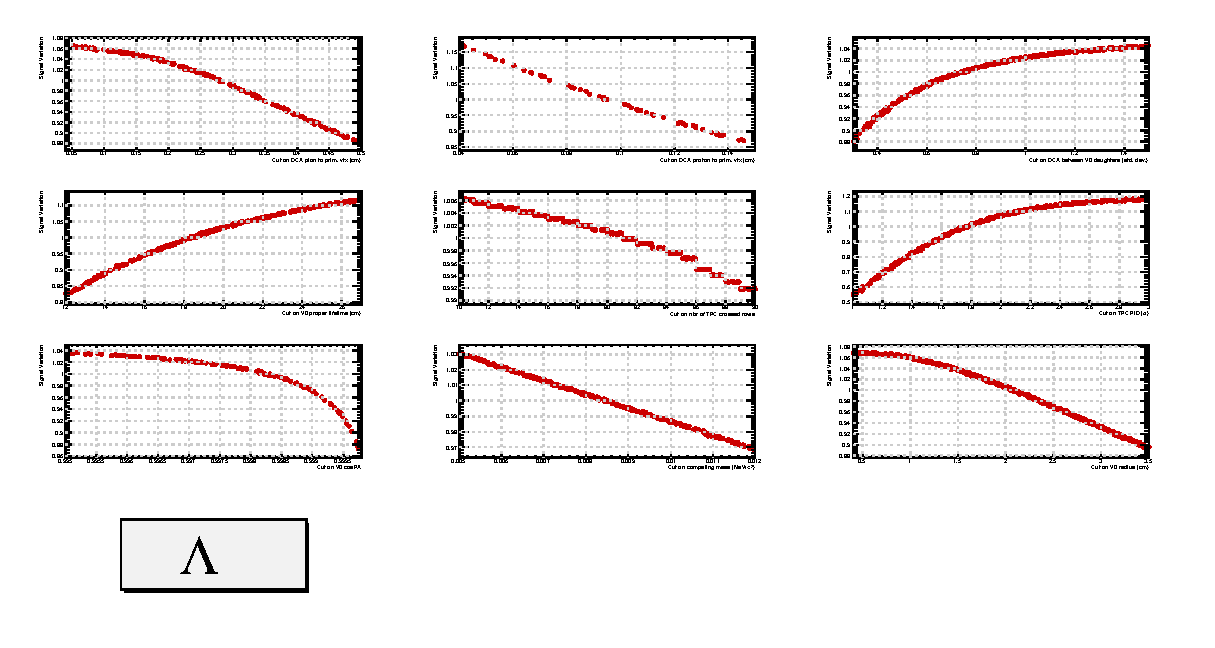
\includegraphics[width=1.45\textwidth]{Figs/Chapter5/SignalVariation_Lambda.eps}
\caption{Signal variation within the selection range of every topological and track variables used in the \rmLambda analysis. These distributions were obtained by fixing all the cuts to their values in \tab\ref{tab:V0Selections} but one; the procedure in \Sec\ref{subsubsec:SystTopoMass} is then used to vary randomly the latter within its range of selections (see \tab\ref{tab:SystematicSelectionsLambda}). The ratio between the extracted signal and the average signal within the selection range provides the signal variation. Here, the signal was computed based on the fit of the invariant mass using a modified Gaussian for the peak and a first order polynomial for the background.}
	\label{fig:SignalVariation_TopoSel_Lambda}
\end{figure}

\begin{figure}[h]
	\centering
	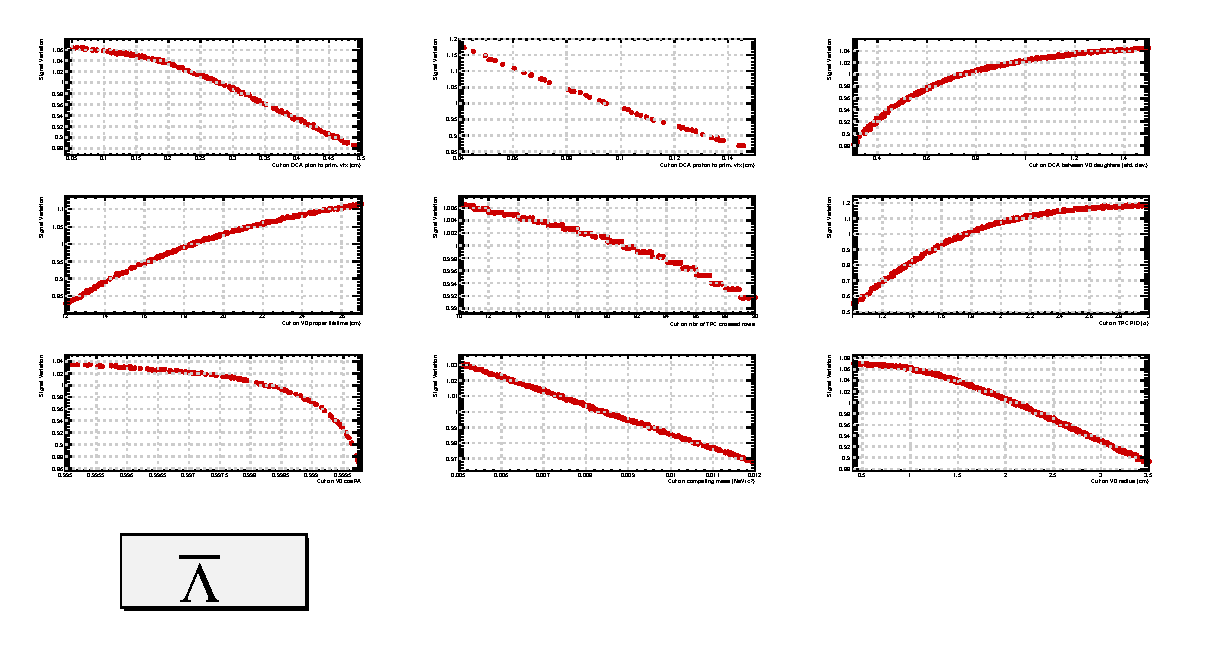
\includegraphics[width=1.45\textwidth]{Figs/Chapter5/SignalVariation_AntiLambda.eps}
\caption{Signal variation within the selection range of every topological and track variables used in the \rmAlambda analysis. These distributions were obtained by fixing all the cuts to their values in \tab\ref{tab:V0Selections} but one; the procedure in \Sec\ref{subsubsec:SystTopoMass} is then used to vary randomly the latter within its range of selections (see \tab\ref{tab:SystematicSelectionsLambda}). The ratio between the extracted signal and the average signal within the selection range provides the signal variation. Here, the signal was computed based on the fit of the invariant mass using a modified Gaussian for the peak and a first order polynomial for the background.}
	\label{fig:SignalVariation_TopoSel_AntiLambda}
\end{figure}

\begin{figure}[h]
	\centering
	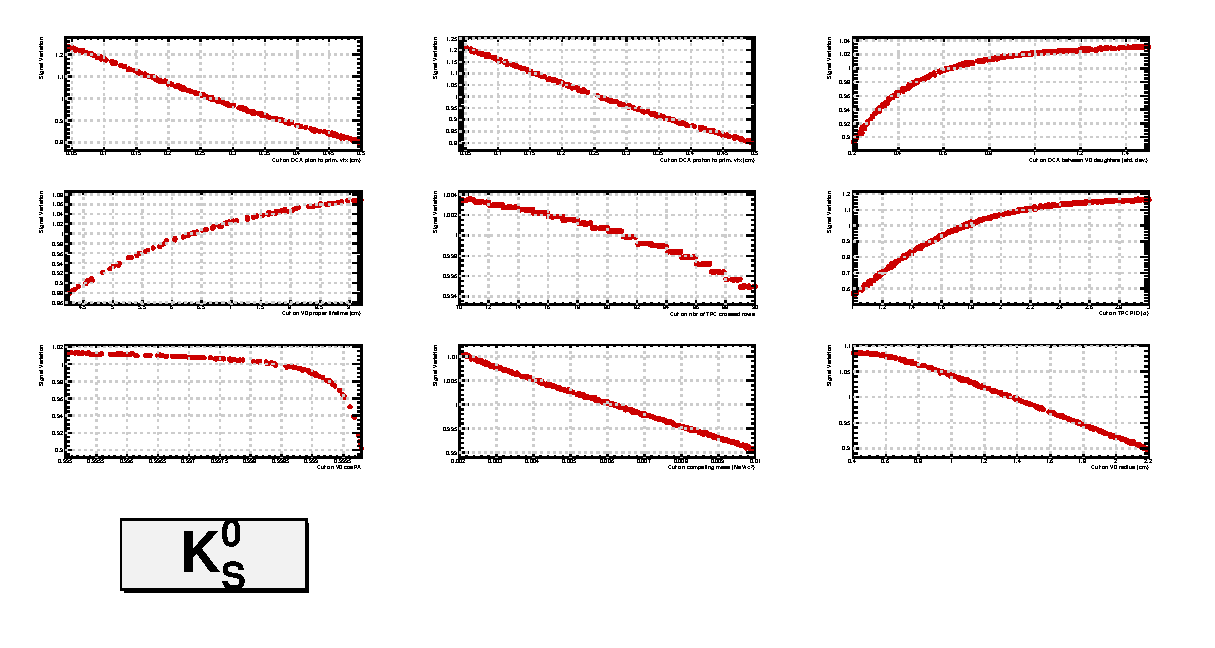
\includegraphics[width=1.45\textwidth]{Figs/Chapter5/SignalVariation_K0s.eps}
\caption{Signal variation within the selection range of every topological and track variables used in the \rmKzero analysis. These distributions were obtained by fixing all the cuts to their values in \tab\ref{tab:V0Selections} but one; the procedure in \Sec\ref{subsubsec:SystTopoMass} is then used to vary randomly the latter within its range of selections (see \tab\ref{tab:SystematicSelectionsK0s}). The ratio between the extracted signal and the average signal within the selection range provides the signal variation. Here, the signal was computed based on the fit of the invariant mass using a modified Gaussian for the peak and a first order polynomial for the background.}
	\label{fig:SignalVariation_TopoSel_K0s}
\end{figure}
\end{landscape}

\section{Summary of the systematic uncertainties}

\begin{table}[H]
    \centering
    \begin{tabular}{c|c|c}
    \noalign{\smallskip}\hline \noalign{\smallskip}
    \bf  & \multicolumn{2}{c}{Uncertainties on the measured mass (\mmass)} \\
    \bf Sources & \multicolumn{2}{c}{\rmKzeroS}\\
    \bf  & Statistical & Systematic \\
    \noalign{\smallskip}\hline \noalign{\smallskip}
    Topological selections & 0.022 & 0.013 \\
    Momentum calibration & / & 0.229\\
    Magnetic field & / & 0.080 \\
    Material budget & / & 0.052\\
    Fitting function & / & 0.006 \\
    Fitting range & / & 0.001 \\    
    Binning & / & 0.001\\
    Out-of-bunch pile-up rejection & / & 0.029 \\
    Precision on the PDG mass & / & negligible\\
    MC mass offset & / & 0.047\\
    \noalign{\smallskip}\hline \noalign{\smallskip}
    \bf Total &\bf 0.022 &\bf 0.256\\
    \noalign{\smallskip}\hline \noalign{\smallskip}
    \end{tabular}
    \caption{Statistical and systematical uncertainties on the mass \rmKzeroS. The total is obtained assuming that there is no correlation between each source of uncertainties.}\label{tab:SystMassK0s}
\end{table}

\begin{table}[H]
    \centering
    \begin{tabular}{c|c|c|c|c}
    \noalign{\smallskip}\hline \noalign{\smallskip}
    \bf  & \multicolumn{4}{c}{Uncertainties on the measured mass (\mmass)} \\
    \bf Sources & \multicolumn{2}{c|}{\rmLambda} & \multicolumn{2}{c}{\rmAlambda}\\
    \bf  & Statistical & Systematic & Statistical & Systematic\\
    \noalign{\smallskip}\hline \noalign{\smallskip}
    Topological selections & 0.011 & 0.006 & 0.011 & 0.004\\
    Momentum calibration & / & 0.056 & / & 0.056 \\
    Magnetic field & / & 0.013 & / & 0.013 \\
    Material budget & / & 0.020 & / & 0.020 \\
    Fitting function & / & 0.009 & / & 0.009\\
    Fitting range & / & 0.001 & / & 0.001 \\    
    Binning & / & 0.001 & / & 0.001 \\
    Out-of-bunch pile-up rejection & / & 0.004 & / & 0.004 \\
    Precision on the PDG mass & / & negligible & / & negligible \\
    MC mass offset & / & 0.015 & / & 0.015 \\
    \noalign{\smallskip}\hline \noalign{\smallskip}
    \bf Total &\bf 0.011 &\bf 0.066 &\bf 0.011 &\bf 0.065 \\
    \noalign{\smallskip}\hline \noalign{\smallskip}
    \end{tabular}
    \caption{Statistical and systematical uncertainties on the mass \rmLambda and \rmAlambda. The total is obtained assuming that there is no correlation between each source of uncertainties.}\label{tab:SystMassLambda}
\end{table}

\begin{table}[H]
    \centering
    \begin{tabular}{c|c|c}
    \noalign{\smallskip}\hline \noalign{\smallskip}
    \bf  & \multicolumn{2}{c}{Uncertainties on the measured mass difference ($\times 10^{-5}$)} \\
    \bf Sources & \multicolumn{2}{c}{\rmLambda} \\
    \bf  & Statistical & Systematic \\
    \noalign{\smallskip}\hline \noalign{\smallskip}
    Topological selections & 1.34 & 1.31\\
    Momentum calibration & / & negligible \\
    Magnetic field & / & negligible \\
    Material budget & / & negligible\\
    Fitting function & / & 0.69\\
    Fitting range & / & 0.02 \\    
    Binning & / & 0.02 \\
    Out-of-bunch pile-up rejection & / & negligible\\
    Precision on the PDG mass & / & negligible\\
    MC mass offset & / & 1.72 \\
    \noalign{\smallskip}\hline \noalign{\smallskip}
    \bf Total &\bf 1.34 & \bf 2.27 \\
    \noalign{\smallskip}\hline \noalign{\smallskip}
    \end{tabular}
    \caption{Statistical and systematical uncertainties on the mass \rmLambda and \rmAlambda. The total is obtained assuming that there is no correlation between each source of uncertainties.}\label{tab:SystMassDiffLambda}
\end{table}

